\begin{anexosenv}

\partanexos

\chapter{Primeiro Anexo}
\begin{figure}[!h]
    \centering
    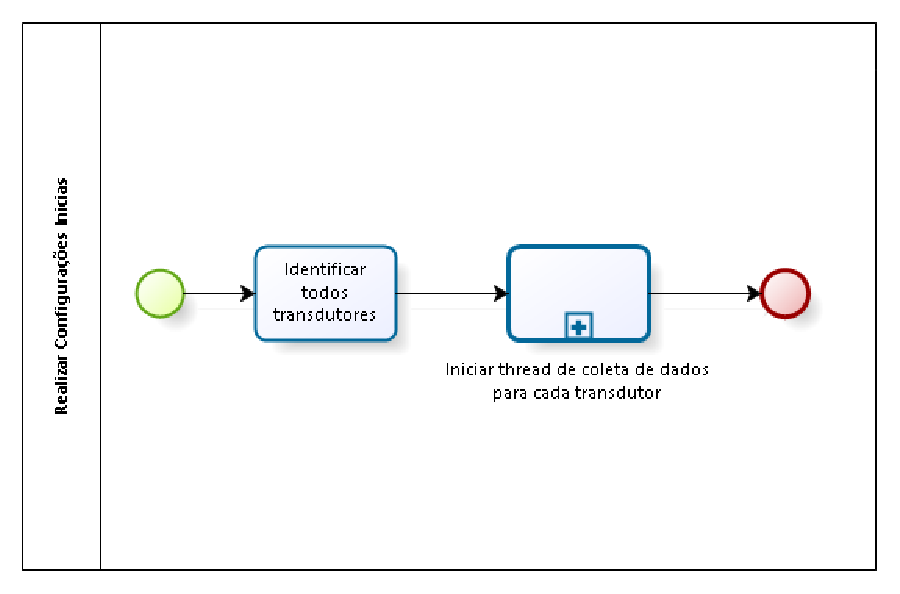
\includegraphics[keepaspectratio=true,scale=1.0]{figuras/process_2.eps}
    \caption{}
    \label{process_2}
\end{figure}

\begin{figure}[!h]
    \centering
    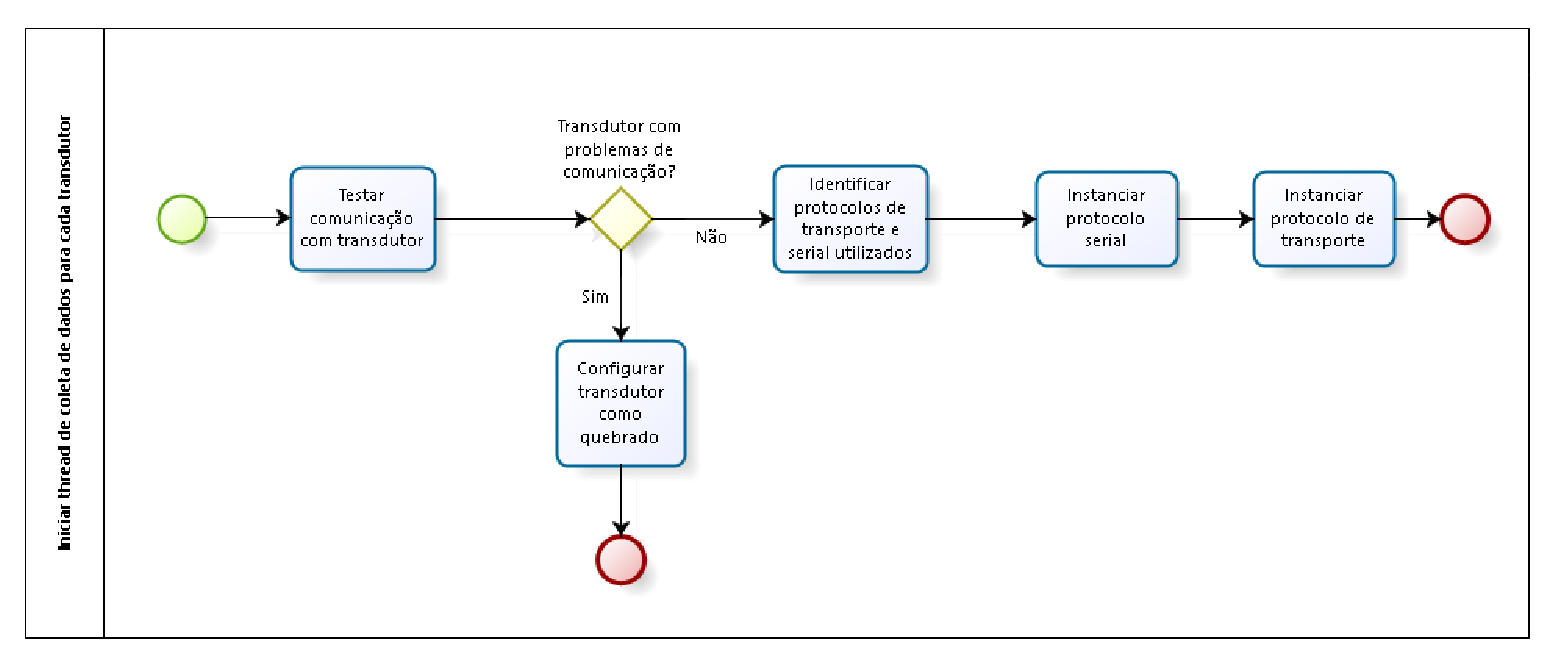
\includegraphics[keepaspectratio=true,scale=0.7,angle=90]{figuras/process_3.eps}
    \caption{}
    \label{process_3}
\end{figure}

\begin{figure}[!h]
    \centering
    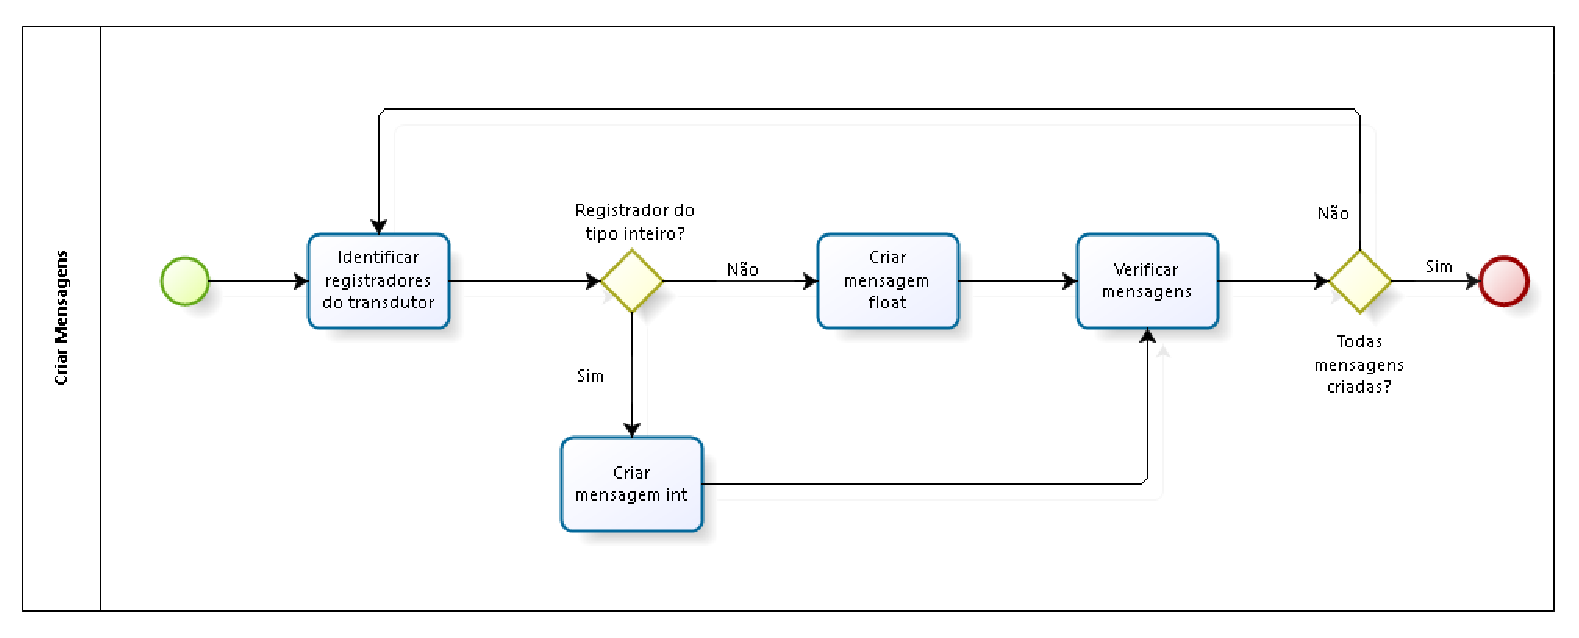
\includegraphics[keepaspectratio=true,scale=0.7,angle=90]{figuras/process_4.eps}
    \caption{}
    \label{process_4}
\end{figure}

\begin{figure}[!h]
    \centering
    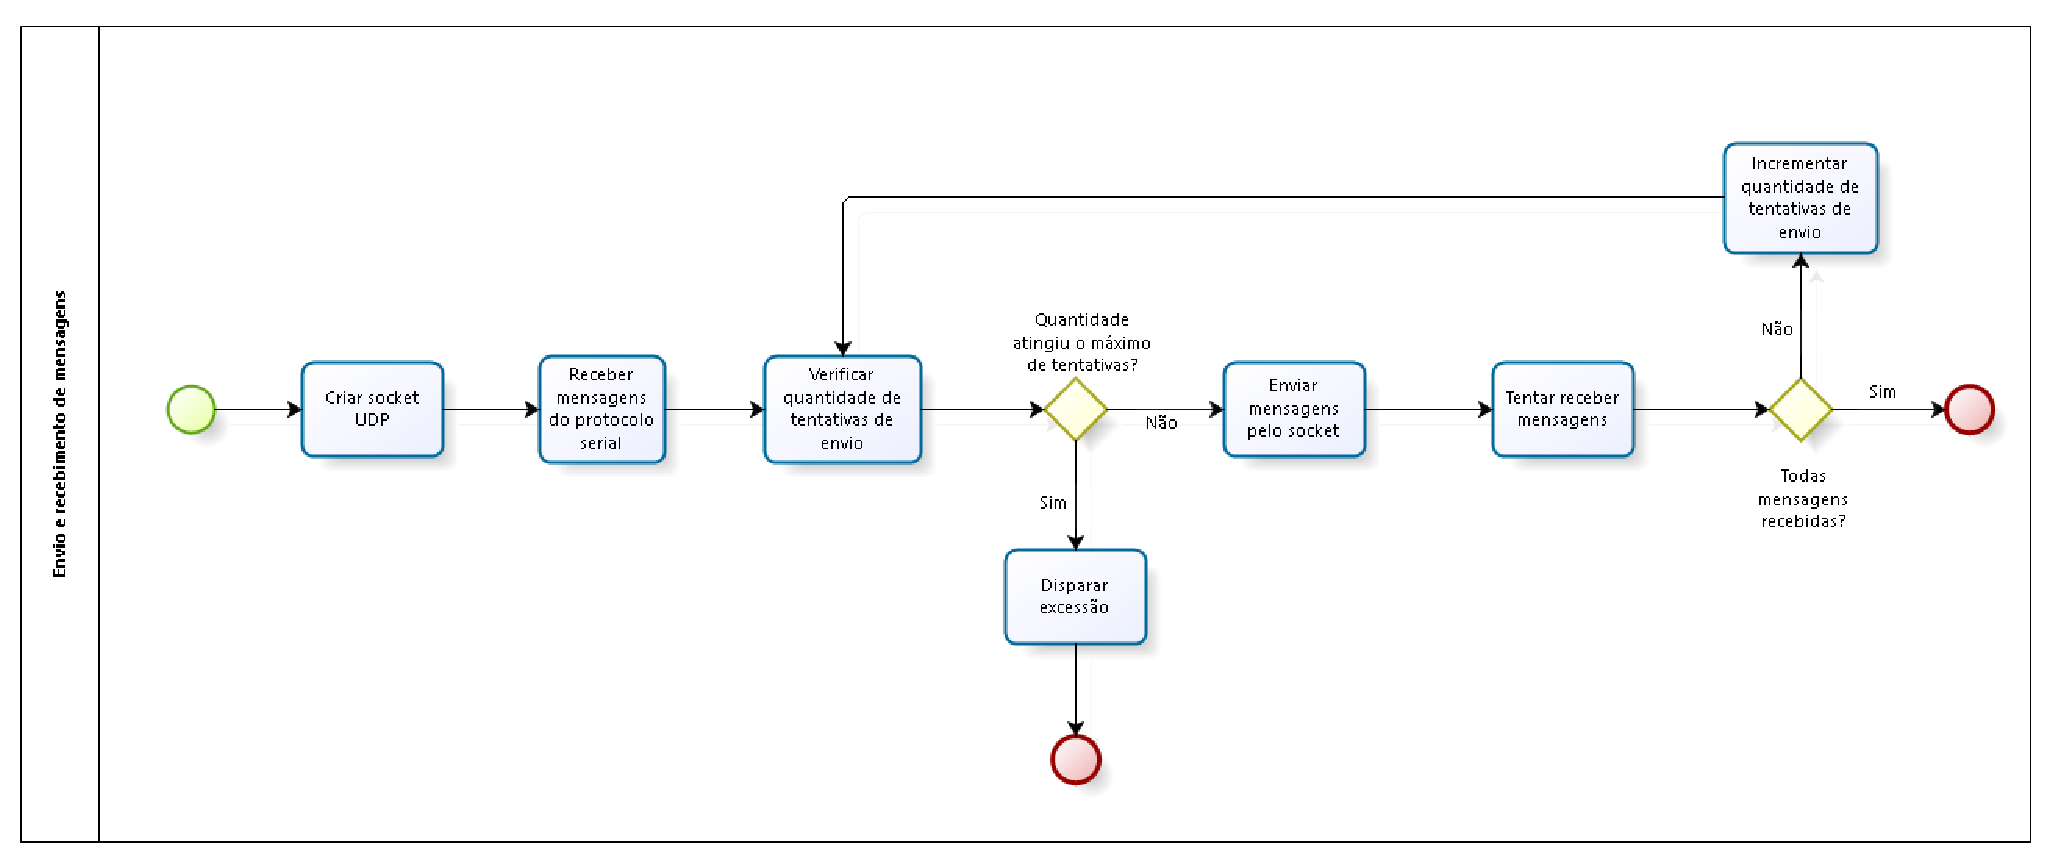
\includegraphics[keepaspectratio=true,scale=0.7,angle=90]{figuras/process_5.eps}
    \caption{}
    \label{process_5}
\end{figure}

\begin{figure}[!h]
    \centering
    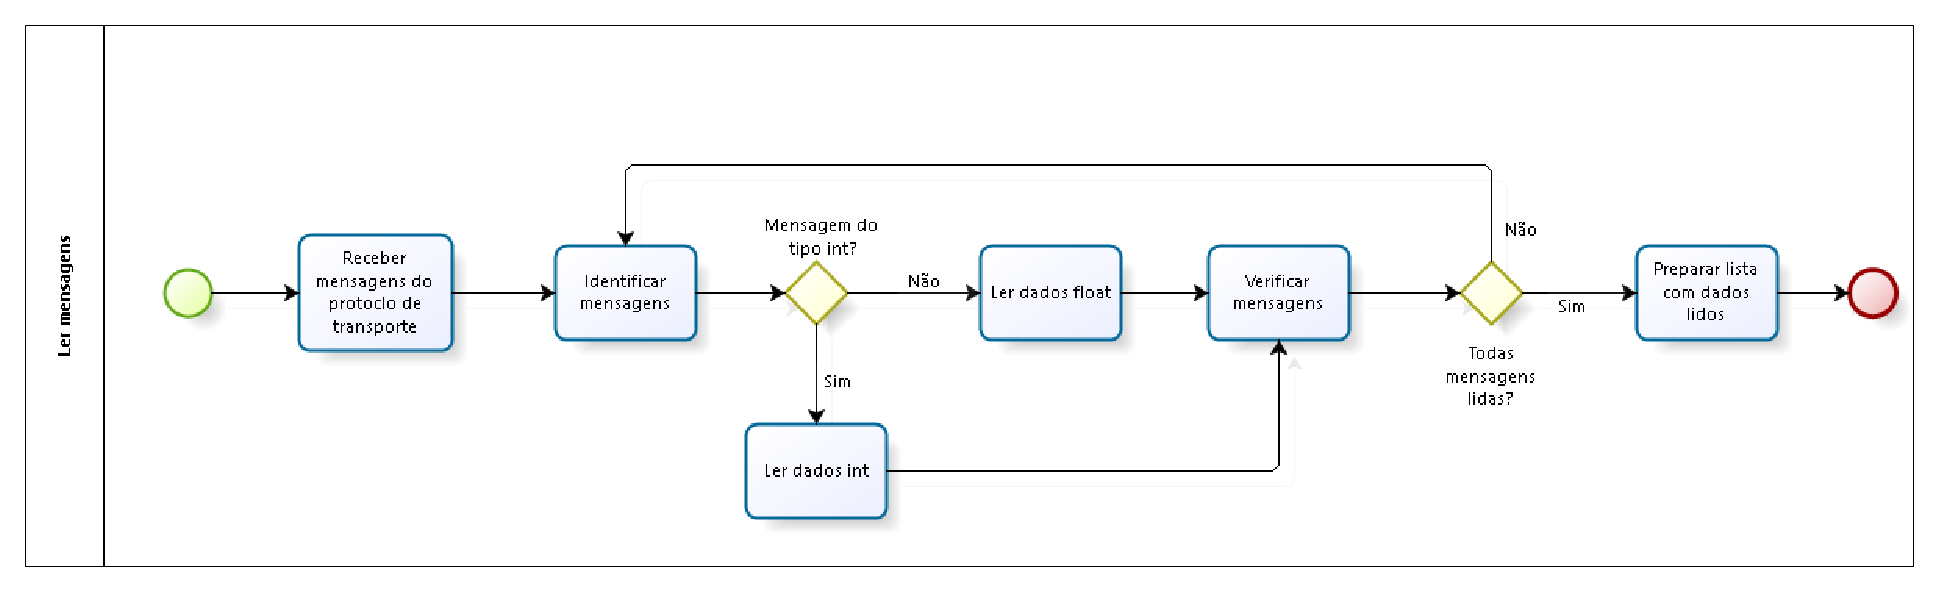
\includegraphics[keepaspectratio=true,scale=0.7,angle=90]{figuras/process_6.eps}
    \caption{}
    \label{process_6}
\end{figure}

\begin{figure}[!h]
    \centering
    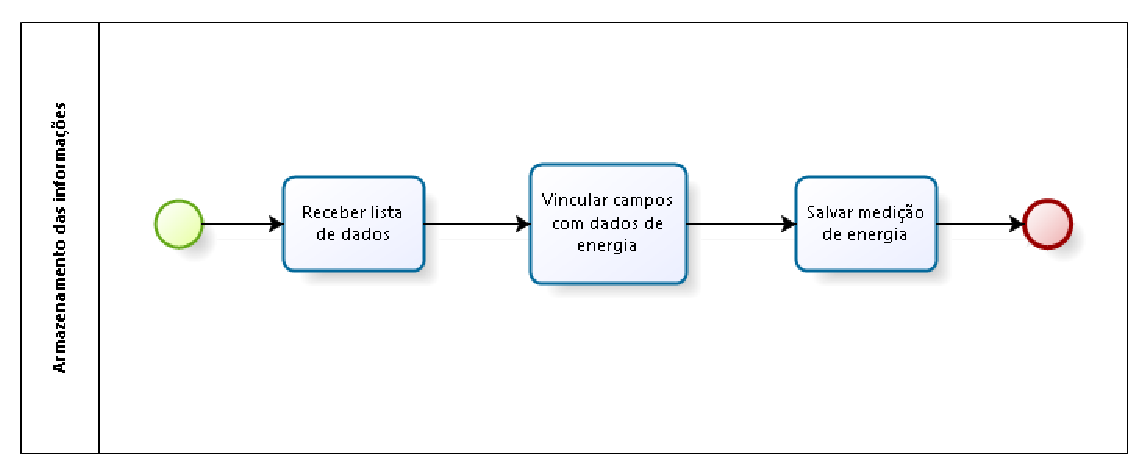
\includegraphics[keepaspectratio=true,scale=1.0]{figuras/process_7.eps}
    \caption{}
    \label{process_7}
\end{figure}

\chapter{Segundo Anexo}

Texto do segundo anexo.

\end{anexosenv}

